\documentclass[sigconf]{acmart}

\usepackage{booktabs} % For formal tables


% Copyright
%\setcopyright{none}
%\setcopyright{acmcopyright}
%\setcopyright{acmlicensed}
\setcopyright{rightsretained}
%\setcopyright{usgov}
%\setcopyright{usgovmixed}
%\setcopyright{cagov}
%\setcopyright{cagovmixed}


% DOI
\acmDOI{10.475/123_4}

% ISBN
\acmISBN{123-4567-24-567/08/06}

%Conference
\acmConference[KDD'17]{ACM Woodstock conference}{August 13 - 17, 2017}{Halifax, Nova Scotia, Canada} 
\acmYear{2017}
\copyrightyear{2017}

\acmPrice{15.00}

\includecomment{kdd}\excludecomment{arxiv}

\begin{document}
\title{Learning rule lists with branch and bound}
\titlenote{Produces the permission block, and
  copyright information}
\subtitle{Extended Abstract}
\subtitlenote{The full version of the author's guide is available as
  \texttt{acmart.pdf} document}


\author{Elaine Angelino}
%\authornote{Dr.~Trovato insisted his name be first.}
%\orcid{1234-5678-9012}
\affiliation{%
  \institution{EECS, UC Berkeley}
  %\streetaddress{}
  \city{Berkeley} 
  \state{CA} 
  \postcode{94720}
}
\email{elaine@eecs.berkeley.edu}

\author{Nicholas Larus-Stone}
%\authornote{The secretary disavows any knowledge of this author's actions.}
\affiliation{%
  \institution{SEAS, Harvard University}
  %\streetaddress{}
  \city{Cambridge} 
  \state{MA} 
  \postcode{02138}
}
\email{nlarusstone@college.harvard.edu}

\author{Daniel Alabi}
%\authornote{The secretary disavows any knowledge of this author's actions.}
\affiliation{%
  \institution{SEAS, Harvard University}
  %\streetaddress{}
  \city{Cambridge} 
  \state{MA} 
  \postcode{02138}
}
\email{alabid@g.harvard.edu}

\author{Margo Seltzer}
%\authornote{The secretary disavows any knowledge of this author's actions.}
\affiliation{%
  \institution{SEAS, Harvard University}
  %\streetaddress{}
  \city{Cambridge} 
  \state{MA} 
  \postcode{02138}
}
\email{margo@eecs.harvard.edu}

\author{Cynthia Rudin}
\affiliation{%
  \institution{Duke University}
  \city{Durham}
  \state{NC} 
  \postcode{27708}}
\email{cynthia@cs.duke.edu}

% The default list of authors is too long for headers}
\renewcommand{\shortauthors}{E. Angelino et al.}


\begin{abstract}
This paper provides a sample of a \LaTeX\ document which conforms,
somewhat loosely, to the formatting guidelines for
ACM SIG Proceedings\footnote{This is an abstract footnote}. 
\end{abstract}

%
% The code below should be generated by the tool at
% http://dl.acm.org/ccs.cfm
% Please copy and paste the code instead of the example below. 
%
\begin{CCSXML}
<ccs2012>
 <concept>
  <concept_id>10010520.10010553.10010562</concept_id>
  <concept_desc>Computer systems organization~Embedded systems</concept_desc>
  <concept_significance>500</concept_significance>
 </concept>
 <concept>
  <concept_id>10010520.10010575.10010755</concept_id>
  <concept_desc>Computer systems organization~Redundancy</concept_desc>
  <concept_significance>300</concept_significance>
 </concept>
 <concept>
  <concept_id>10010520.10010553.10010554</concept_id>
  <concept_desc>Computer systems organization~Robotics</concept_desc>
  <concept_significance>100</concept_significance>
 </concept>
 <concept>
  <concept_id>10003033.10003083.10003095</concept_id>
  <concept_desc>Networks~Network reliability</concept_desc>
  <concept_significance>100</concept_significance>
 </concept>
</ccs2012>  
\end{CCSXML}

\ccsdesc[500]{Computer systems organization~Embedded systems}
\ccsdesc[300]{Computer systems organization~Redundancy}
\ccsdesc{Computer systems organization~Robotics}
\ccsdesc[100]{Networks~Network reliability}

% We no longer use \terms command
%\terms{Theory}

\keywords{ACM proceedings, \LaTeX, text tagging}

\maketitle

%\documentclass[aoas,preprint]{imsart}
%\usepackage{fullpage}
%\setattribute{journal}{name}{}
%\usepackage[usenames,dvipsnames,svgnames,table]{xcolor}
%
%\usepackage{graphicx,verbatim}
%\usepackage[round]{natbib}
%\usepackage{url}
%\usepackage{amsmath,amssymb,amsthm,amsfonts}
%\usepackage{algorithm}
%\usepackage{algpseudocode}
%\usepackage{todonotes}
%\usepackage{subfig}
%\usepackage{dsfont}
%\usepackage{listings}
%\usepackage{comment}
%
%\usepackage{tikz}
%\usetikzlibrary{arrows}
%
%\newcommand{\eanote}[1]{{\color{magenta} (EA) #1}}
\newcommand{\red}[1]{{\color{red} #1}}
\newcommand{\yellow}[1]{{\color{yellow} #1}}
\newcommand{\green}[1]{{\color{green} #1}}
\newcommand{\eat}[1]{ }

\def\ie{{\it i.e.},~}
\def\eg{{\it e.g.},~}
\def\etal{{\it et al.}~}

\def\E{\mathbb{E}}
\def\P{\mathbb{P}}
\def\Var{\mbox{Var}}
\def\Unif{\mbox{Unif}}
\def\Normal{\mbox{Normal}}
\def\reals{\mathbb{R}}
\def\ints{\mathbb{Z}}
\def\one{\mathds{1}}
\def\Normal{\mathrm{Normal}}
\def\X{{\mathcal X}}
\def\Y{{\mathcal Y}}
\def\RL{{\mathcal R}}
\def\N{{\mathcal N}}
\def\Prefix{{\mathcal P}}
\def\RuleSet{{\mathcal S}}
\newcommand{\x}{\mathbf{x}}
\newcommand{\y}{\mathbf{y}}

\newcommand{\eins}{\mbox{$1 \hspace{-1.0mm} {\bf l}$}}
\newcommand{\A}{\mathcal{A}}
\newcommand{\Ac}{\mathcal{A}^c}
\newcommand{\T}[3]{T_{#1}(#2 \leftarrow #3)}
\def\reals{\mathbb{R}}
\def\one{\mathds{1}}

\newtheorem{lemma}{Lemma}
\newtheorem{theorem}{Theorem}
\newtheorem{remark}{Remark}
\newtheorem{definition}{Definition}
\newtheorem{proposition}{Proposition}
\newtheorem{claim}{Claim}

\newcommand{\noi}{\noindent}
\newcommand{\nn}{\nonumber}
\newcommand{\be}{\begin{equation}}
\newcommand{\ee}{\end{equation}}
\newcommand{\bea}{\begin{eqnarray}}
\newcommand{\eea}{\end{eqnarray}}
\newcommand{\erf}{\text{erf}}
\newcommand{\bits}[1]{\texttt{#1}}

\newcommand{\given}{\,|\,}

%\frenchspacing
%\hyphenation{speed-up}
%
%\begin{document}

\section{Introduction}

As machine learning continues to grow in importance for socially-important decisions, the interpretability of predictive models remains a crucial problem. Our goal is to build models that are both highly predictive and easily understood by humans. We use rule lists, also known as decision lists, to achieve this goal. Rule lists are lists composed of if-then statements, which are easily interpreted; the rules give a reason for each prediction.

Constructing rule lists, or more generally, decision trees, has been a challenge for more than
30 years; most approaches use greedy splitting techniques~\cite{Rivest87,Breiman84,Quinlan93}. 
%
Recent approaches use Bayesian analysis, either to find a locally optimal solution~\cite{Chipman:1998jh} or to explore the search space~\citep{LethamRuMcMa15, YangRuSe16}.
%
These approaches achieve high accuracy while also managing to run reasonably quickly. However, despite the apparent accuracy of the rule lists generated by these algorithms, there is no way to determine either if the generated rule list is optimal or how close it is to optimal.

Optimality is important, because there are societal implications for a lack of optimality.
%
Consider the recent ProPublica article on the COMPAS recidivism prediction tool~\citep{LarsonMaKiAn16}.
%
It highlights a case where a black-box, proprietary predictive model is being used for recidivism prediction.
%
The authors show that the COMPAS scores are racially biased, but since the model is not transparent, no one (outside of the creators of COMPAS) can determine the reason or extent of the bias~\citep{LarsonMaKiAn16}, nor can anyone determine the reason for any particular prediction.
%
By using COMPAS, users implicitly assumed that a transparent model
would not be sufficiently accurate for recidivism prediction,
\ie they assumed that a black box model would provide better accuracy.
%
We wondered whether there was indeed no possible transparent model that would suffice.
%
Answering that question requires solving a computationally hard problem.
%
Namely, we would like to find a transparent model that is optimal
within a particular pre-determined class of models,
and produce a certificate of optimality.
%
This would enable one to say, for this problem and model class,
with certainty and before resorting to black box methods,
whether there exists a transparent model.

To that end, we consider the class of rule lists created from pre-mined frequent itemsets.
%
The rule list must be assembled from these itemsets to minimize a regularized risk function,~$R$.
%
This is a hard discrete optimization problem.
%
Brute force solutions that minimize~$R$ are computationally prohibitive
due to the exponential number of possible rule lists.
%
However, this is a worst case bound that is not realized in practical settings.
%
For realistic cases, it is possible to solve fairly large cases of this problem to optimality,
with the careful use of algorithms, data structures, and implementation techniques.

We develop specialized tools from the field of discrete optimization and artificial intelligence, and in particular, a special branch-and-cut algorithm, called  Certifiably Optimal RulE ListS (CORELS), that provides (1) the optimal solution, (2) a certficiate of optimality and (3) a collection of near-optimal solutions and the distance between each such solution and the optimal one. The certificate of optimality means that we can investigate how close other models (e.g., models provided by greedy algorithms) are to optimal. In particular, we can investigate if the rule lists from probabilistic approaches are nearly optimal or whether those approaches sacrifice too much accuracy in the interest of speed.

\begin{arxiv}
Within its branch-and-cut procedure, CORELS maintains an upper bound on the maximum value of $R$ that each incomplete rule list can achieve. This allows it to prune an incomplete rule list (and every possible extension) if the bound is worse than the accuracy of the best rule list that we've already looked at. The use of careful bounding techniques leads to massive pruning of the search space of potential rule lists. We continue to consider incomplete and complete rule lists until we have either examined or eliminated every rule list from consideration. Thus, we terminate with the optimal rule list, the close-to-optimal rule lists, and a certificate of optimality.
\end{arxiv}

The efficacy of CORELS depends on how much of the search space our bounds allow us to prune. The upper bound on $R$ must thus be as tight as reasonably possible. The bound we maintain throughout the calculation is a minimum of several bounds, that come in three categories. The first category of bounds are those intrinsic to the rules themselves. This category includes bounds stating that each rule must capture sufficient data; if not, the rule list is provably non-optimal. The second type of bound compares an upper bound on the value of $R$ to that of the current best solution. This allows us to exclude parts of the search space that could never be better than our current solution. Finally, our last type of bound is based on comparing incomplete rule lists that capture the same data and pursuing only the more accurate option. This last class of bounds is especially important -- without our use of a novel \textit{symmetry-aware map}, we are unable to solve most problems of reasonable scale. This symmetry-aware map keeps track of the best accuracy for all the permutations of a given incomplete rule list.

We keep track of these bounds using a modified \emph{prefix tree},
a data structure also known as a trie.
%
Each node in the prefix tree represents an individual rule;
thus, each path in the tree represents a rule list such that
the final node in the path contains metrics about that rule list.
%
This tree structure facilitates the use of multiple different selection algorithms including breadth-first search, a priority queue whose priority metric is customizable, and a stochastic selection process. In addition, we are able to limit the number of nodes in the tree and thereby achieve a way of tuning space-time tradeoffs in a robust manner. This tree structure is a useful way of organizing the generation of rule lists and should be parallelizable.

\begin{arxiv}
We evaluated CORELS on a number of publicly available datasets and have made code for our algorithm and experiments publicly available. Our metric of success was 10-fold cross validated prediction accuracy on a subset of the data. These datasets involve hundreds of rules and hundreds or thousands of observations. CORELS is generally able to find the optimal rule list in a matter of seconds and certify it within about 10 minutes. We show that we are able to achieve better out-of-sample accuracy on these datasets than the popular greedy algorithms, CART and C5.0.
\end{arxiv}

With CORELS, we target large (not massive) problems,
where interpretability and certifiable optimality are important.
%
We illustrate the efficacy of our approach using the ProPublica COMPAS dataset~\cite{LarsonMaKiAn16}, for predicting two-year recidivism.
%
We produce a certifiably optimal, interpretable rule list that achieves
the same accuracy as a random forest approach, thereby calling into question
the need for use of a proprietary, black box algorithm for recidivism prediction.

%\bibliographystyle{abbrvnat}
%\bibliography{refs}
%
%\end{document}


%\documentclass[aoas,preprint]{imsart}
%\usepackage{fullpage}
%\setattribute{journal}{name}{}
%\usepackage[usenames,dvipsnames,svgnames,table]{xcolor}
%
%\usepackage{graphicx,verbatim}
%\usepackage[round]{natbib}
%\usepackage{url}
%\usepackage{amsmath,amssymb,amsthm,amsfonts}
%\usepackage{algorithm}
%\usepackage{algpseudocode}
%\usepackage{todonotes}
%\usepackage{subfig}
%\usepackage{dsfont}
%\usepackage{listings}
%\usepackage{comment}
%
%\usepackage{tikz}
%\usetikzlibrary{arrows}
%
%\newcommand{\eanote}[1]{{\color{magenta} (EA) #1}}
\newcommand{\red}[1]{{\color{red} #1}}
\newcommand{\yellow}[1]{{\color{yellow} #1}}
\newcommand{\green}[1]{{\color{green} #1}}
\newcommand{\eat}[1]{ }

\def\ie{{\it i.e.},~}
\def\eg{{\it e.g.},~}
\def\etal{{\it et al.}~}

\def\E{\mathbb{E}}
\def\P{\mathbb{P}}
\def\Var{\mbox{Var}}
\def\Unif{\mbox{Unif}}
\def\Normal{\mbox{Normal}}
\def\reals{\mathbb{R}}
\def\ints{\mathbb{Z}}
\def\one{\mathds{1}}
\def\Normal{\mathrm{Normal}}
\def\X{{\mathcal X}}
\def\Y{{\mathcal Y}}
\def\RL{{\mathcal R}}
\def\N{{\mathcal N}}
\def\Prefix{{\mathcal P}}
\def\RuleSet{{\mathcal S}}
\newcommand{\x}{\mathbf{x}}
\newcommand{\y}{\mathbf{y}}

\newcommand{\eins}{\mbox{$1 \hspace{-1.0mm} {\bf l}$}}
\newcommand{\A}{\mathcal{A}}
\newcommand{\Ac}{\mathcal{A}^c}
\newcommand{\T}[3]{T_{#1}(#2 \leftarrow #3)}
\def\reals{\mathbb{R}}
\def\one{\mathds{1}}

\newtheorem{lemma}{Lemma}
\newtheorem{theorem}{Theorem}
\newtheorem{remark}{Remark}
\newtheorem{definition}{Definition}
\newtheorem{proposition}{Proposition}
\newtheorem{claim}{Claim}

\newcommand{\noi}{\noindent}
\newcommand{\nn}{\nonumber}
\newcommand{\be}{\begin{equation}}
\newcommand{\ee}{\end{equation}}
\newcommand{\bea}{\begin{eqnarray}}
\newcommand{\eea}{\end{eqnarray}}
\newcommand{\erf}{\text{erf}}
\newcommand{\bits}[1]{\texttt{#1}}

\newcommand{\given}{\,|\,}

%\frenchspacing
%\hyphenation{speed-up}
%
%\begin{document}

\section{Related Work}


We discuss related literature in several subfields.

\textit{Interpretable Models:} There is a growing interest in interpretable (transparent, comprehensible) models because of their societal importance~\citep[see ][]{ruping2006learning,bratko1997machine,dawes1979robust,VellidoEtAl12,Giraud98,Holte93,Schmueli10,Huysmans11,Freitas14}. There are now regulations on algorithmic decision-making in the European Union on the ``right to an explanation" \citep{Goodman2016EU} that would legally require interpretability in predictions.


\textit{Optimal Decision Tree Modeling}: The body of work closest to ours is possibly that of optimal decision tree modeling. There is work starting in the late 1990's on building optimal decision trees using optimization techniques \citep{Bennett96optimaldecision,dobkininduction}, continuing until the present \citep{FarhangfarGZ08}. 
A particularly interesting paper along these lines is that of \citet{NijssenFromont2010}, who created a ``bottom-up" way to form optimal decision trees. Their method performs an expensive search step, mining all possible leaves (rather than all possible rules), and uses those leaves to form trees. Their method can lead to memory problems, but it is possible that these memory issues can be mitigated using the theorems in this paper. \footnote{There is no public version of their code for distribution as of this writing.} Another work close to ours is that of \citet{GarofalakisHyRaSh00}, who introduce an algorithm to generate more interpretable decision trees by allowing constraints to be placed on the size of the decision tree. During tree construction, they bound the possible Minimum Description Length (MDL) cost of every different split at a given node. If every split at that node is more expensive than the actual cost of the current subtree, then that node can be pruned. In this way, they are able to prune the tree while constructing it instead of just constructing the tree and then pruning at the end. They do not aim for optimal trees; they build trees that obey constraints, and find optimal subtrees within the trees that were built during the building phase.
%\textcolor{red}{Hm?} However, even with the added bounds, this approach does not generally yield globally optimal decision trees because they constrained the number of nodes in the tree.

\textit{Greedy splitting and pruning:} Unlike optimal decision tree methods, methods like
CART \citep{Breiman84} and C4.5 \citep{Quinlan93} do not perform exploration of the search space beyond greedy splitting. There are a huge number of algorithms in this class.

\textit{Bayesian tree and rule list methods}: Some of these methods that aim to explore the space of trees \citep{Dension:1998hl,Chipman:2002hc,Chipman10} using Monte Carlo exploration methods, however, the space of trees of a given depth is much larger than the space of rule lists of that same level of depth, and the trees within these algorithms are grown in a top-down greedy way. Because of this, the authors noted that the MCMC chain tends to reach only locally optimal solutions. This explains why Bayesian rule-based methods \citep{LethamRuMcMa15,YangRuSe16} have tended to be more successful in escaping local minima. Our work builds specifically on that of \citet{YangRuSe16}. In particular, we use their efficient bit-vector representation and build on their bounds. Note that the 1995 RIPPER algorithm \cite{ripper} is similar to the Bayesian tree methods in that it grows, prunes, and then locally optimizes.

\textit{Rule learning methods:} 
Most rule learning methods are not designed for optimality or interpretability, but for computational speed and/or accuracy. In \textit{associative classification} \citep{Vanhoof10,Liu98,Li01,Yin03}, classifiers are often formed greedily from the top down as rule lists, or they are formed by taking the simple union of pre-mined rules, whereby any observation that fits into any of the rules is classified as positive. In \textit{inductive logic programming} \citep{muggleton1994inductive}, algorithms form disjunctive normal form patterns via a set of operations (rather than using optimization). These approaches are not appropriate for obtaining a guarantee of optimality. Methods for decision list learning construct rule lists iteratively in a greedy way
\citep{Rivest87,Sokolova03,Marchand05,RudinLeMa13,Goessling2015}, which again have no guarantee on optimality, and tend not to produce optimal rule lists in general. Some methods allow for interpretations of single rules, without constructing rule lists \citep{McCormick:2011ws}.

There is a tremendous amount of related work in other subfields that are too numerous to discuss at length here. We have not discussed \textit{rule mining} algorithms since they are part of an interchangeable preprocessing step for our algorithm and are deterministically fast (that is, they will not generally slow our algorithm down). We also did not discuss methods that create disjunctive normal form models, e.g., logical analysis of data, and many associative classification methods. 

\textit{Related problems with interpretable lists of rules:} Beyond trees that are optimized for accuracy and sparsity, rule lists have been developed that have exotic types of constraints, and for various applications.
For example, Falling Rule Lists \citep{WangRu15} are constrained to have decreasing probabilities down the list as are rule lists for dynamic treatment regimes \citep{ZhangEtAl15} and cost-sensitive dynamic treatment regimes \citep{LakkarajuRu17}. Both Wang et. al \cite{WangRu15} and Lakkaraju et. al \cite{LakkarajuRu17} use Monte Carlo searches through the space of rule lists. The method proposed in this work could potentially be adapted to handle these kinds of interesting problems. We are currently working on bounds for Falling Rule Lists \citep{ChenRu17} similar to those presented here.




%	Recent work in the field of decision lists has focused on the creation of probabilistic decision lists that generate a posterior distribution over the space of potential decision lists\citep{LethamRuMcMa15,YangRuSe16}. These methods achieve good accuracy while maintaining a small execution time. In addition, these methods improve on existing methods such as CART or C5.0 by optimizing over the global space of decision lists as opposed to searching for rules greedily and getting stuck at local optima. We take the same approach towards optimizing over the global search space, though we don’t use probabilistic techniques. In addition, we use the rule mining framework from \citep{LethamRuMcMa15} to generate the rules for our data sets. \citep{YangRuSe16} builds on \citep{LethamRuMcMa15} by placing bounds on the search space and creating a high performance bit vector manipulation library. We use that bit vector manipulation library to perform our computations, and add additional bounds to further prune the search space.




%Efficient Algorithms for Constructing Decision Trees with Constraints, Scalable Data Mining with Model Constraints, Building Decision Trees with Constraints

%	Our use of a branch and bound technique has also been applied to decision tree generation methods. \citep{garofalakis:2000-kdd} created an algorithm to generate more interpretable decision trees by allowing one to constrain the size of the decision tree. \citep{garofalakis:2000-kdd} uses branch-and-bound to constrain the size of the search space and limit the eventual size of the decision tree. During tree construction, \citep{garofalakis:2000-kdd} bounds the possible MDL cost of every different split at a given node. If every split at that node is more expensive than the actual cost of the current subtree, then that node can be pruned. In this way, they were able to prune the tree while constructing it instead of just constructing the tree and then pruning at the end.

%ProPublica
%	Certain problems require that the model used to solve that problem be interpretable as well as accurate. \citep{LarsonMaKiAn16} examines the problem of predicting recidivism and shows that a black box model, specifically the COMPAS score from the company Northpointe, has racially biased prediction. Black defendants are misclassified at a higher risk for recidivism than in actuality, while white defendants are misclassified at a lower risk. The model which produces the COMPAS scores is a black box algorithm which is not interpretable, and therefore the model does not provide a way for human input to correct for these racial biases. Our model produces similar accuracies to the logistic regression and COMPAS scores from \citep{LarsonMaKiAn16} while maintaining its interpretability.

%\bibliographystyle{abbrvnat}
%\bibliography{refs}
%
%\end{document}


\section{Implementation}
\label{sec:implementation}

\subsection{Incremental computation}
\label{sec:incremental}

For every prefix~$\Prefix$ evaluated during
Algorithm~\ref{alg:branch-and-bound}'s execution, we compute
the objective lower bound~${b(\Prefix, \x, \y)}$ and, sometimes,
the objective~${\Obj(\RL, \x, \y)}$ of the corresponding rule list~$\RL$.
%
These calculations are the dominant computations with respect to execution time.
%
This motivates our use of a highly optimized library,
designed by~\citet{YangRuSe16} for representing rule lists and
performing operations encountered in evaluating functions of rule lists.
%
Furthermore, we exploit the hierarchical nature of the objective
function and its lower bound to compute these quantities
incrementally throughout branch-and-bound execution.
%
\begin{arxiv}
In this section, we provide explicit expressions for
the incremental computations that are central to our approach.
\end{arxiv}
%
Later, in~\S\ref{sec:implementation}, we describe a cache data structure
for supporting our incremental framework in practice.

\begin{arxiv}
For completeness, before presenting our incremental expressions,
let us begin by writing down the objective lower bound and objective
of the empty rule list, ${\RL = ((), (), \Default, 0)}$,
the first rule list evaluated in Algorithm~\ref{alg:branch-and-bound}.
%
Since its prefix contains zero rules, it has zero prefix
misclassification error and also has length zero.
%
Thus, the empty rule list's objective lower bound is zero:
\begin{align}
  b((), \x, \y) = \Loss_p((), (), \x, \y) + \Reg \cdot 0 = 0.
\end{align}
%
Since none of the data are captured by the empty prefix, the default rule
corresponds to the majority class, and the objective corresponds to the
default rule misclassification error, \ie
\begin{align}
  \Obj(\RL, \x, \y) = \Loss(\RL, \x, \y) + \Reg \cdot 0
  &= \Loss_p((), (), \x, \y) + \Loss_0((), \Default, \x, \y) \nn \\
  &= b((), \x, \y) + \Loss_0((), \Default, \x, \y) = \Loss_0((), \Default, \x, \y).
\end{align}

Now, we derive our incremental expressions for the objective function and its lower bound.
%
Let ${\RL = (\Prefix, \Labels, \Default, K)}$ and
${\RL' = (\Prefix', \Labels', \Default', K + 1)}$
be rule lists such that prefix ${\Prefix = (p_1, \dots, p_K)}$
is the parent of ${\Prefix' = (p_1, \dots, p_K, p_{K+1})}$.
%
Let ${\Labels = (q_1, \dots, q_K)}$ and
${\Labels' = (q_1, \dots, q_K, q_{K+1})}$ be the corresponding labels.
%
The hierarchical structure of Algorithm~\ref{alg:branch-and-bound}
enforces that if we ever evaluate~$\RL'$, then we will have already
evaluated both the objective and objective lower bound of its parent,~$\RL$.
%
We would like to reuse as much of these computations as possible
in our evaluation of~$\RL'$.
%
We can write the objective lower bound of~$\RL'$ incrementally,
with respect to the objective lower bound of~$\RL$:
\begin{align}
b(\Prefix', \Labels', \x, \y)
  &= \Loss_p(\Prefix', \Labels', \x, \y) + \Reg (K + 1) \nn \\
&= \frac{1}{N} \sum_{n=1}^N \sum_{k=1}^{K+1} \Cap(x_n, p_k \given \Prefix')
  \wedge \one [ q_k \neq y_n ] + \Reg (K+1) \label{eq:non-inc-lb} \\
&= \Loss_p(\Prefix, \Labels, \x, \y) + \Reg K + \Reg
  + \frac{1}{N} \sum_{n=1}^N \Cap(x_n, p_{K+1} \given \Prefix') \wedge \one [q_{K+1} \neq y_n ] \nn \\
&= b(\Prefix, \Labels, \x, \y) + \Reg
  + \frac{1}{N} \sum_{n=1}^N \Cap(x_n, p_{K+1} \given \Prefix') \wedge \one [q_{K+1} \neq y_n ] \nn \\
&= b(\Prefix, \Labels, \x, \y) + \Reg  + \frac{1}{N} \sum_{n=1}^N \neg\, \Cap(x_n, \Prefix) \wedge
  \Cap(x_n, p_{K+1}) \wedge \one [q_{K+1} \neq y_n].
\label{eq:inc-lb}
\end{align}
%Notice that the term~${\neg\, \Cap(x_n, \Prefix)}$ in~\eqref{eq:inc-lb}
%depends only on~$\Prefix$, \ie it does not depend on~$\Prefix'$; furthermore,
%it is computed in the evaluation of~$\RL$'s default rule misclassification error,
%\begin{align}
%\Loss_0(\Prefix, \Default, \x, \y) = \frac{1}{N}\sum_{n=1}^N \neg\, \Cap(x_n, \Prefix) \wedge \one [q_0 \neq y_n].
%\end{align}
Thus, if we store $b(\Prefix, \Labels, \x, \y)$, % and ${\neg\, \Cap(\x, \Prefix)}$,
then we can reuse this quantity when computing $b(\Prefix', \Labels', \x, \y)$.
%
Transforming~\eqref{eq:non-inc-lb} into~\eqref{eq:inc-lb} yields a
significantly simpler expression that is a function of the stored
quantity~$b(\Prefix, \Labels, \x, \y)$. %, as well as ${\neg\, \Cap(\x, \Prefix)}$
%and the last rule of~$\RL'$, ${p_{K+1} \rightarrow q_{K+1}}$.
%
For the objective of~$\RL'$, first let us write a na\"ive expression:
\begin{align}
\Obj(\RL', \x, \y) &= \Loss(\RL', \x, \y) + \Reg (K + 1)
= \Loss_p(\Prefix', \Labels', \x, \y) + \Loss_0(\Prefix', \Default', \x, \y) + \Reg(K + 1) \nn \\
&= \frac{1}{N} \sum_{n=1}^N \sum_{k=1}^{K+1} \Cap(x_n, p_k \given \Prefix')
  \wedge \one [ q_k \neq y_n ] + \frac{1}{N}\sum_{n=1}^N \neg\, \Cap(x_n, \Prefix') \wedge
  \one [q'_0 \neq y_n] + \Reg (K+1). \label{eq:non-inc-obj}
\end{align}
Instead, we can compute the objective of~$\RL'$ incrementally
with respect to its objective lower bound:
\begin{align}
\Obj(\RL', \x, \y) &=  \Loss_p(\Prefix', \Labels', \x, \y) +
  \Loss_0(\Prefix', \Default', \x, \y) + \Reg (K + 1) \nn \\
&= b(\Prefix', \Labels', \x, \y) + \Loss_0(\Prefix', \Default', \x, y) \nn \\
&= b(\Prefix', \Labels', \x, \y) + \frac{1}{N}\sum_{n=1}^N \neg\, \Cap(x_n, \Prefix') \wedge
  \one [q'_0 \neq y_n] \nn \\
&= b(\Prefix', \Labels', \x, \y) + \frac{1}{N}\sum_{n=1}^N \neg\, \Cap(x_n, \Prefix) \wedge
  (\neg\, \Cap(x_n, p_{K+1})) \wedge \one [q'_0 \neq y_n].
\label{eq:inc-obj}
\end{align}
The expression in~\eqref{eq:inc-obj} is much simpler than the na\"ive
one in~\eqref{eq:non-inc-obj}, and is a function of
$b(\Prefix', \Labels', \x, \y)$, which we computed in~\eqref{eq:inc-lb}.
%as well as ${\neg\, \Cap(\x, \Prefix)}$,
%and the last antecedent~$p_{K+1}$ and default rule~$\Default'$ of~$\RL'$.
Though we could compute the objective of~$\RL'$ incrementally
with respect to that of~$\RL$, doing so would in practice require
that we also store~$\Obj(\RL, \x, \y)$; we prefer the approach suggested
by~\eqref{eq:inc-obj} since it avoids this additional storage overhead.

\begin{algorithm}[t!]
  \caption{Incremental branch-and-bound for learning rule lists, for simplicity, from a cold start.
  We explicitly show the incremental objective lower bound and objective functions in Algorithm~\ref{alg:incremental-functions}.}
\label{alg:incremental}
\begin{algorithmic}
\normalsize
\State \textbf{Input:} Objective function~$\Obj(\RL, \x, \y)$,
objective lower bound~${b(\Prefix, \x, \y)}$,
set of antecedents ${\RuleSet = \{s_m\}_{m=1}^M}$,
training data~$(\x, \y) = {\{(x_n, y_n)\}_{n=1}^N}$,
regularization parameter~$\Reg$
\State \textbf{Output:} Provably optimal rule list~$\OptimalRL$ with minimum objective~$\OptimalObj$ \\

\State $\CurrentRL \gets ((), (), \Default, 0)$ \Comment{Initialize current best rule list with empty rule list}
\State $\CurrentObj \gets \Obj(\CurrentRL, \x, \y)$ \Comment{Initialize current best objective}
\State $Q \gets $ queue$(\,[\,(\,)\,]\,)$ \Comment{Initialize queue with empty prefix}
\State $C \gets $ cache$(\,[\,(\,(\,)\,, 0\,)\,]\,)$ \Comment{Initialize cache with empty prefix and its objective lower bound}
\While {$Q$ not empty} \Comment{Optimization complete when the queue is empty}
	\State $\Prefix \gets Q$.pop(\,) \Comment{Remove a prefix~$\Prefix$ from the queue}
        \State $b(\Prefix, \x, \y) \gets C$.find$(\Prefix)$ \Comment{Look up $\Prefix$'s lower bound in the cache}
        \State $\mathbf{u} \gets \neg\,\Cap(\x, \Prefix)$ \Comment{Bit vector indicating data not captured by $\Prefix$}
        \For {$s$ in $\RuleSet$} \Comment{Evaluate all of $\Prefix$'s children}
            \If {$s$ not in $\Prefix$}
                \State $\PrefixB \gets (\Prefix, s)$ \Comment{\textbf{Branch}: Generate child $\PrefixB$}
                \State $\mathbf{v} \gets \mathbf{u} \wedge \Cap(\x, s)$ \Comment{Bit vector indicating data captured by $s$ in $\PrefixB$}
                \State $b(\PrefixB, \x, \y) \gets b(\Prefix, \x, \y) + \Reg~ + $ \Call{IncrementalLowerBound}{$\mathbf{v}, \y, N$} \Comment{Eq.~\eqref{eq:inc-lb}}
                \If {$b(\PrefixB, \x, \y) < \CurrentObj$} \Comment{\textbf{Bound}: Apply bound from Theorem~\ref{thm:bound}}
                    \State $\Obj(\RLB, \x, \y) \gets b(\PrefixB, \x, \y)~ + $ \Call{IncrementalObjective}{$\mathbf{u}, \mathbf{v}, \y, N$} \Comment{Eq.~\eqref{eq:inc-obj}}
                    \If {$\Obj(\RLB, \x, \y) < \CurrentObj$}
                        \State $(\CurrentRL, \CurrentObj) \gets (\RLB, \Obj(\RLB, \x, \y))$ \Comment{Update current best rule list and objective}
                    \EndIf
                    \State $Q$.push$(\PrefixB)$ \Comment{Add $\PrefixB$ to the queue}
                    \State $C$.insert$(\PrefixB, b(\PrefixB, \x, \y))$ \Comment{Add $\PrefixB$ and its lower bound to the cache}
                \EndIf
            \EndIf
        \EndFor
\EndWhile
\State $(\OptimalRL, \OptimalObj) \gets (\CurrentRL, \CurrentObj)$ \Comment{Identify provably optimal rule list and objective}
\end{algorithmic}
\end{algorithm}

\begin{algorithm}[t!]
  \caption{Incremental objective lower bound~\eqref{eq:inc-lb} used in Algorithm~\ref{alg:incremental}.}
\label{alg:incremental-lb}
\begin{algorithmic}
\normalsize
\State \textbf{Input:}
Bit vector~${\mathbf{v} \in \{0, 1\}^N}$ indicating data captured by $s$, the last antecedent in~$\PrefixB$,
bit vector of class labels~${\y \in \{0, 1\}^N}$,
number of observations~$N$
\State \textbf{Output:} Component of~$\RLB$'s misclassification error due to data captured by~$s$ \\

\Function{IncrementalLowerBound}{$\mathbf{v}, \y, N$}
    \State $n_v = \Count(\mathbf{v})$ \Comment{Number of data captured by $s$, the last antecedent in $\PrefixB$}
    \State $\mathbf{w} \gets \mathbf{v} \wedge \y$ \Comment{Bit vector indicating data captured by $s$ with label $1$}
    \State $n_w = \Count(\mathbf{w})$ \Comment{Number of data captured by $s$ with label $1$}
    \If {$n_w / n_v > 0.5$}
        \State \Return $(n_v - n_w) / N$ \Comment{Misclassification error of the rule $s \rightarrow 1$}
    \Else
        \State \Return $n_w / N$ \Comment{Misclassification error of the rule $s \rightarrow 0$}
    \EndIf
    \EndFunction
\end{algorithmic}
\end{algorithm}

\begin{algorithm}[t!]
  \caption{Incremental objective function~\eqref{eq:inc-obj} used in Algorithm~\ref{alg:incremental}.}
\label{alg:incremental-obj}
\begin{algorithmic}
\normalsize
\State \textbf{Input:}
Bit vector~${\mathbf{u} \in \{0, 1\}^N}$ indicating data not captured by~$\PrefixB$'s parent prefix,
bit vector~${\mathbf{v} \in \{0, 1\}^N}$ indicating data not captured by $s$, the last antecedent in~$\PrefixB$,
bit vector of class labels~${\y \in \{0, 1\}^N}$,
number of observations~$N$
\State \textbf{Output:} Component of~$\RLB$'s misclassification error due to its default rule \\

 \Function{IncrementalObjective}{$\mathbf{u}, \mathbf{v}, \y, N$}
    \State $\mathbf{f} \gets \mathbf{u} \wedge \neg\,\mathbf{v} $ \Comment{Bit vector indicating data not captured by $\PrefixB$}
    \State $n_f = \Count(\mathbf{f})$ \Comment{Number of data not captured by $\PrefixB$}
    \State $\mathbf{g} \gets \mathbf{f} \wedge \y$ \Comment{Bit vector indicating data not captured by $\PrefixB$ with label $1$}
    \State $n_g = \Count(\mathbf{w})$ \Comment{Number of data not captued by $\PrefixB$ with label $1$}
    \If {$n_f / n_g > 0.5$}
        \State \Return $(n_f - n_g) / N$ \Comment{Default rule misclassification error with label $1$}
    \Else
        \State \Return $n_g / N$ \Comment{Default rule misclassification error with label $0$}
    \EndIf
\EndFunction
\end{algorithmic}
\end{algorithm}

We present an incremental branch-and-bound procedure in
Algorithm~\ref{alg:incremental}, and show the incremental computations
of the objective lower bound~\eqref{eq:inc-lb} and objective~\eqref{eq:inc-obj}
as two separate functions in Algorithms~\ref{alg:incremental-lb}
and~\ref{alg:incremental-obj}, respectively.
%
In Algorithm~\ref{alg:incremental}, we use a cache to store
prefixes and their objective lower bounds.
%
Algorithm~\ref{alg:incremental} additionally reorganizes the structure
of Algorithm~\ref{alg:branch-and-bound} to group together the computations
associated with all children of a particular prefix.
%
This has two advantages.
%
The first is to consolidate cache queries: all children of the same
parent prefix compute their objective lower bounds with respect to
the parent's stored value, and we only require one cache `find' operation
for the entire group of children, instead of a separate query for each child.
%
The second is to shrink the queue's size:
instead of adding all of a prefix's children as separate queue elements,
we represent the entire group of children in the queue by a single element.
%
Since the number of children associated with each prefix
is close to the total number of possible antecedents,
both of these effects can yield significant savings.
%
For example, if we are trying to optimize over rule lists formed
from a set of 1000 antecedents, then the maximum queue size in
Algorithm~\ref{alg:incremental} will be smaller than that in
Algorithm~\ref{alg:branch-and-bound} by a factor of nearly 1000.

\end{arxiv}


We implement our algorithm using a collection of optimized data structures:
a trie, a symmetry-aware map, and a queue.
The trie acts like a cache, keeping track of rule lists we have already evaluated.
Each node in the trie contains metadata associated with that corresponding rule list;
the metadata consists of bookkeeping information such as what child rule lists are feasible and
the lower bound and accuracy for that rule list.
The trie also tracks the best observed rule list by keeping track of the minimum objective
found and its associated rule list.

We implement the symmetry-aware map using the C++ STL unordered\_map, which
% Since we are not yet doing anything with the capture-based representation, we shouldn't
% discuss it as we won't be showing performance.
% We have two different versions of the map.
% Both versions 
maps all permutations of a set of rules to a key, whose value
contains the best ordering of those rules (\ie the one with the smallest objective).
Every rule has a rule id number, and we call the numerically sorted order of a set of rules its
canonical order, thus, by quering a set of rules by its canonical order, all
permutations map to the same key.
% Keys in one version of the map represent the set of rules (in canonical order) comprising a
% rule list prefix.
% Keys in the other version represent the set of captured data points.
% The set of captured entries is identical for a given set of rules, independent of ordering, so
% different permutations still map to the same key.
%
% Note that encodings of rule lists in canonical order tend to be
% significantly smaller than encodings of captured data points,
% especially for large datasets.
%
In general, the symmetry-aware map dominates memory usage during long runs.
Before inserting permutation $P_i$ into the symmetry-aware map, we check
if there exists a permutation $P_j$ of $P_i$ already in the map.
If the objective of $P_i$ is better than the objective of $P_j$,
we update the map and remove $P_j$ and its subtree from the trie.
Otherwise we do nothing (\ie we do not insert $P_i$ into the symmetry-aware map
or the trie).

We use a queue to store all of the leaves of the trie that still need to be explored.
We order entries in the queue to implement several different scheduling policies,
including BFS, DFS, and a priority queue, ordered by the lower bound, the objective, or the
curiosity.
We also have a stochastic exploration process that bypasses the use of a queue by walking
the trie, randomly choosing a child each time, until encountering a leaf.
We find that ordering by curiosity often leads to a shorter runtime than using BFS.

Mapping our algorithm to our data structures produces the following execution strategy.
While there are still leaves of the trie to be explored, use the scheduling policy to select
the next rule list to evaluate.
Then, for every rule that is not already in this rule list, we calculate the lower bound,
objective, and other metrics produced if the rule were appended to the rule list.
If the new rule list produces a lower bound less than the current minimum objective, we insert that
rule list into the symmetry-aware map, the tree, and the queue and, if necessary, update the
current minimum objective.
If the lower bound is greater than the minimum objective, meaning this new rule list is never
better than one we have already seen, we do not insert the new rule list into the tree or queue. 

Each time we update the minimum objective, we garbage collect the trie, by walking it
from the root the leaves, deleting any subtrees of nodes with a lower bound larger than the current
minimum objective. If we encounter a node with no children, we prune upwards--deleting that
node and recursively traversing the tree towards the root, deleting any childless nodes.
This garbage collection allows us to constrain the trie's memory consumption, though in our
experiments we observe the minimum objective to decrease only a small number of times.

%\section{Implementation architecture}
%
%We present an architecture for executing our branch-and-bound algorithm,
%consisting of a cache, a queue that is associated with a search policy,
%and, optionally, a symmetry-aware map.
%%
%First, we describe the cache, our primary data structure~(\S\ref{sec:cache});
%it is organized as a prefix tree and supports the incremental computations,
%detailed in~\S\ref{sec:incremental}, that are central to our approach.
%%
%Second, we describe the queue and search policy~(\S\ref{sec:queue}).
%%
%Like the queue in Algorithm~\ref{alg:branch-and-bound},
%our queue keeps track of which prefixes to evaluate during execution.
%%
%The policy for selecting a prefix from the queue to evaluate next,
%and thus also the natural queue data structure, depend on
%the search policy employed for exploring the space of rule lists
%%
%Next, we describe the symmetry-aware map~(\S\ref{sec:map}),
%which enables garbage collection of prefixes eliminated by the
%equivalent support bound in Theorem~\ref{sec:equivalent}.
%%
%While we present the map as an optional component of our architecture,
%our calculations in~\S\ref{sec:permutation-counting}
%and experiments in~\S\ref{sec:experiments} demonstrate that
%it is critical for efficient and practical algorithm performance.
%%
%Finally, we summarize an artifact we implemented~(\S\ref{sec:system}),
%which we evaluate in~\S\ref{sec:experiments}.
%
%\subsection{Prefix tree cache for incremental computation}
%\label{sec:cache}
%
%We maintain a cache to support incremental computation.
%%
%Our cache is organized as a prefix tree, which is also known as a trie.
%%
%
%\subsection{Queue and search policies}
%\label{sec:queue}
%
%Different search policies suggest different natural queue data structures.
%
%\begin{itemize}
%\item breadth-first
%\item depth-first
%\item something based on greedy
%\item (curiosity, lower bound, optimization) $\times$ (priority queue, something like Thompson sampling)
%\item optimistic
%\end{itemize}
%
%\subsection{Map data structure for symmetry-aware garbage collection}
%\label{sec:map}
%
%%\subsection{Large-scale optimization}
%
%\subsection{System}
%\label{sec:system}


\section{Preliminary experiments}
\label{sec:experiments}

\begin{figure}[t!]
\begin{center}
%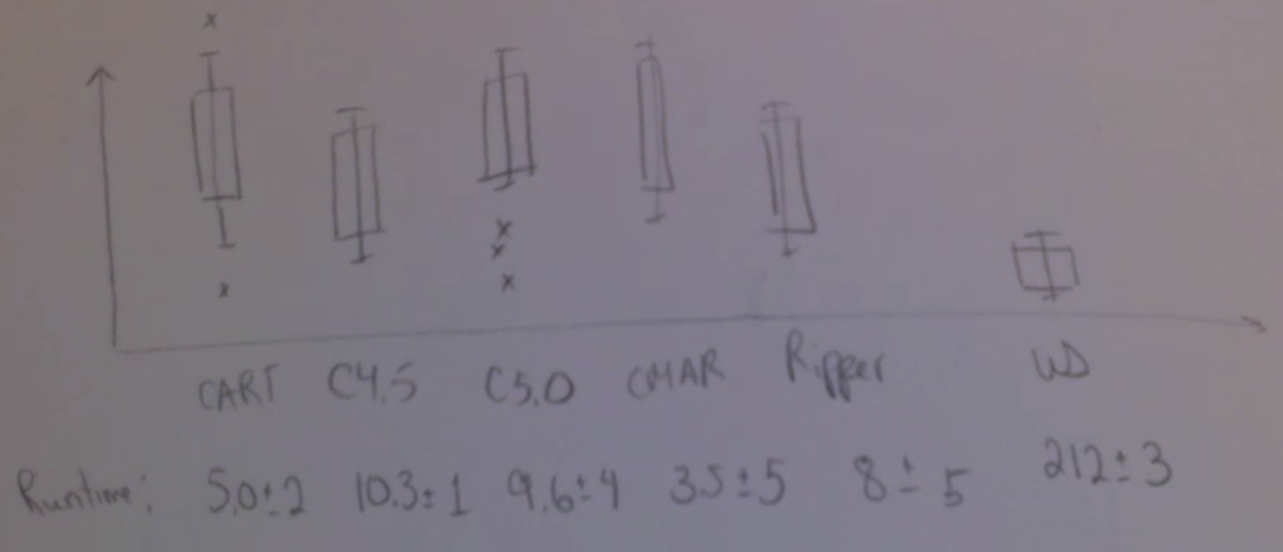
\includegraphics[width=0.75\textwidth]{figs/sketch-comparison.png}
\begin{arxiv}
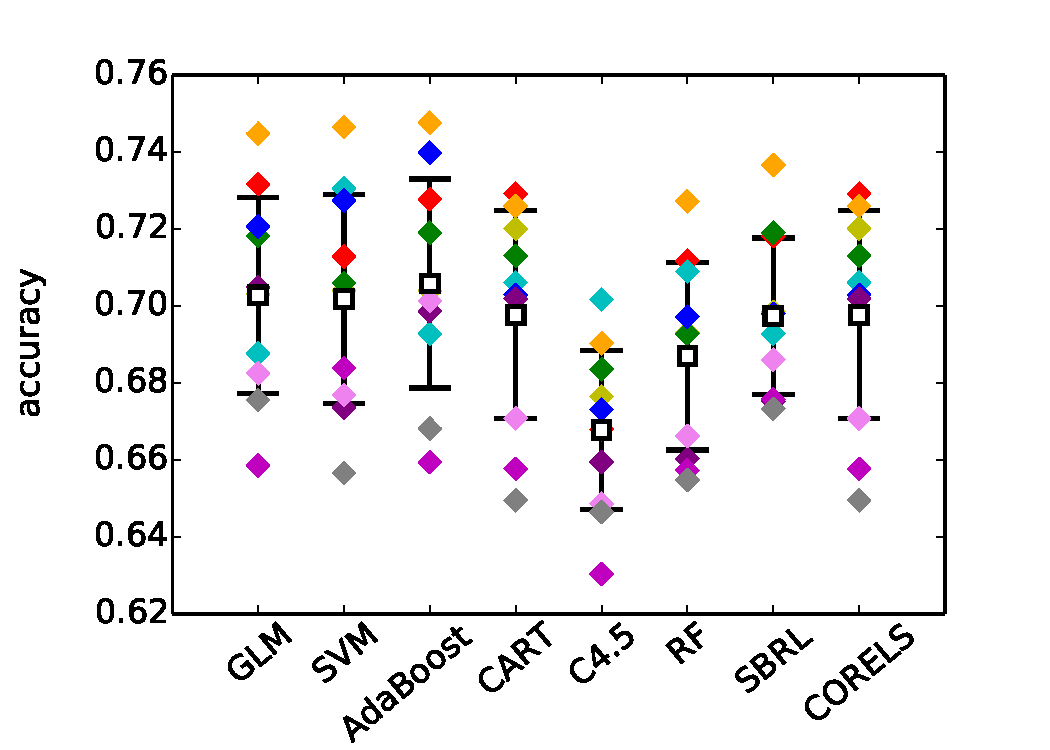
\includegraphics[width=0.75\textwidth]{figs/compare-compas.pdf}
\end{arxiv}
\begin{kdd}
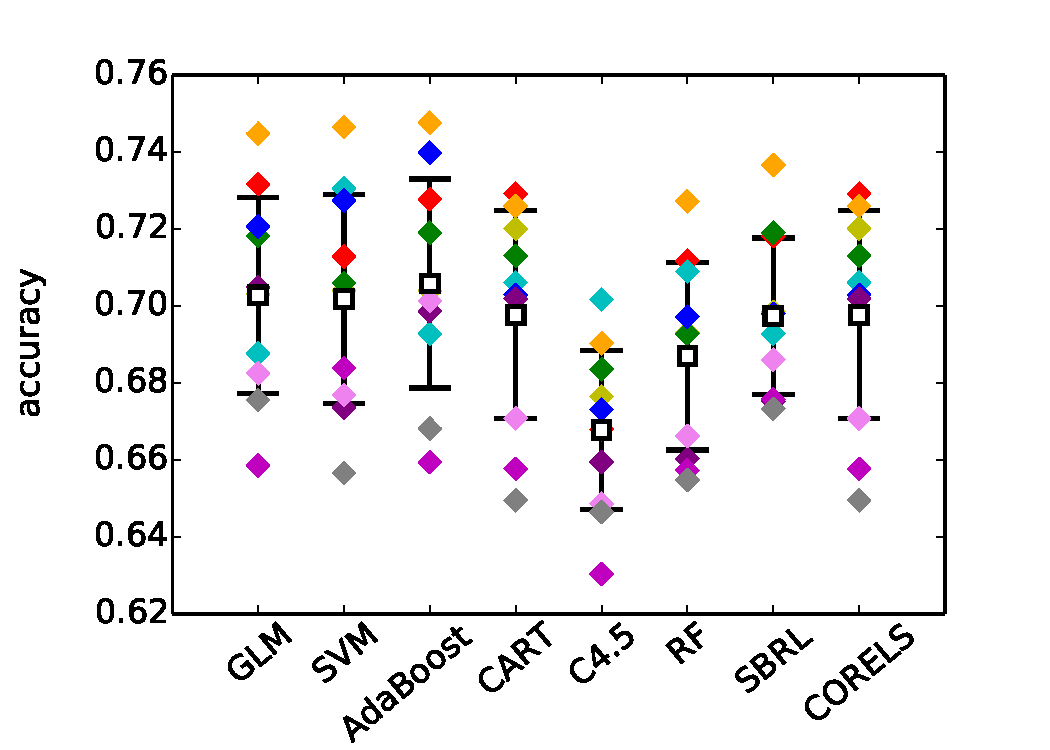
\includegraphics[width=0.5\textwidth]{figs/compare-compas.pdf}
\end{kdd}
\end{center}
\caption{Comparison with other methods:
Test error for us and a few other algorithms
(CART, C4.5, CBA, CMAR/CPAR, C5.0, Ripper, \dots),
as a function of sparsity over 10 folds, for one big dataset (box plots).
Also report algorithm runtimes (mean $\pm$ standard deviation over 10 folds).}
\label{fig:comparison}
\end{figure}

\begin{arxiv}
\begin{figure}[t!]
\begin{center}
\end{center}
\caption{Missing:  Test error as a function of regularization and sparsity
(number of rules) as a function of regularization, over 10 folds,
for one big dataset.}
\label{fig:regularization}
\end{figure}
\end{arxiv}

\begin{arxiv}
\begin{figure}[t!]
\begin{center}
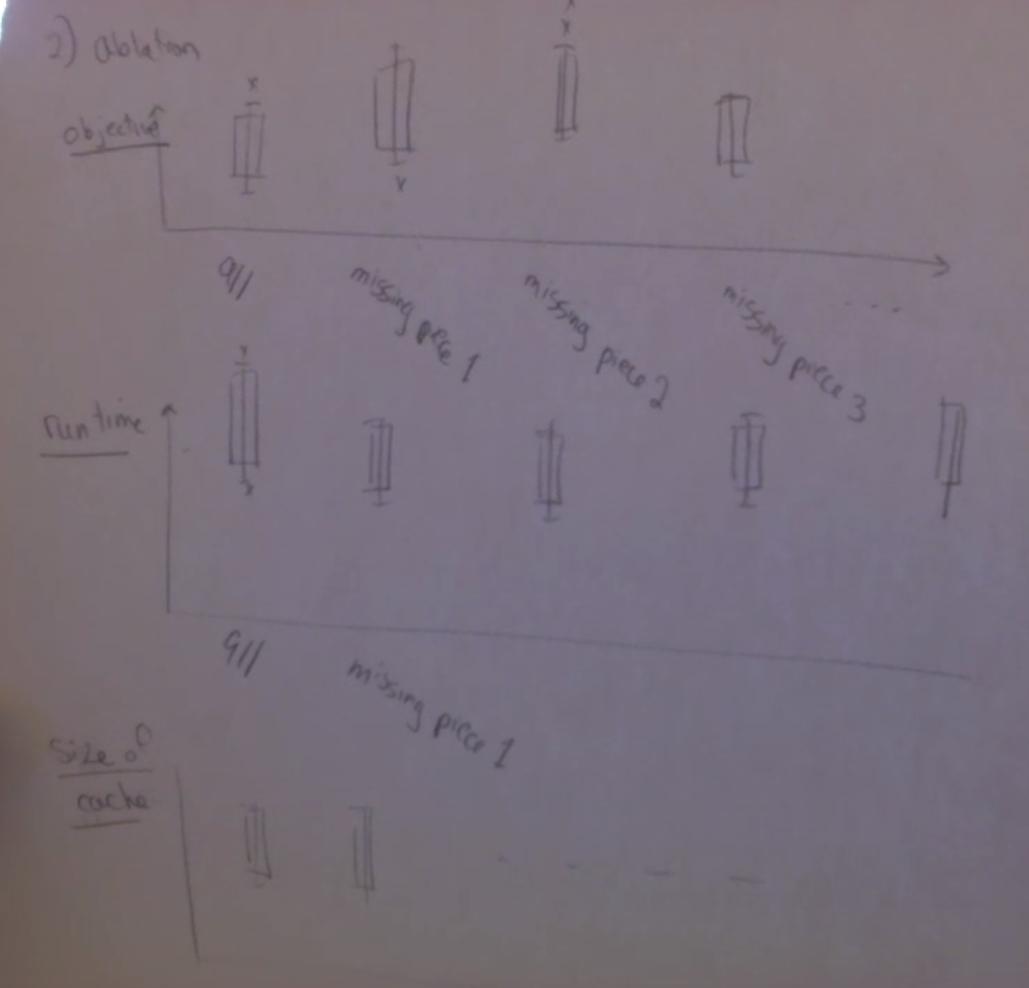
\includegraphics[width=0.75\textwidth]{figs/sketch-ablation.png}
\end{center}
\caption{Ablation experiment:
Show the effect of each ``piece'' at a time,
run X without each in turn and show the difference in either
quality of solution or runtime or amount of memory, size of cache or queue,
where X is a specific implementation
(meaning a specific scheduling policy and node type)}
\label{fig:ablation}
\end{figure}
\end{arxiv}

\begin{arxiv}
\begin{figure}[t!]
\begin{center}
\end{center}
\caption{Missing:  Some sort of comparison of different scheduling policies}
\label{fig:scheduling-policy}
\end{figure}
\end{arxiv}

\begin{arxiv}
\begin{figure}[t!]
\begin{center}
%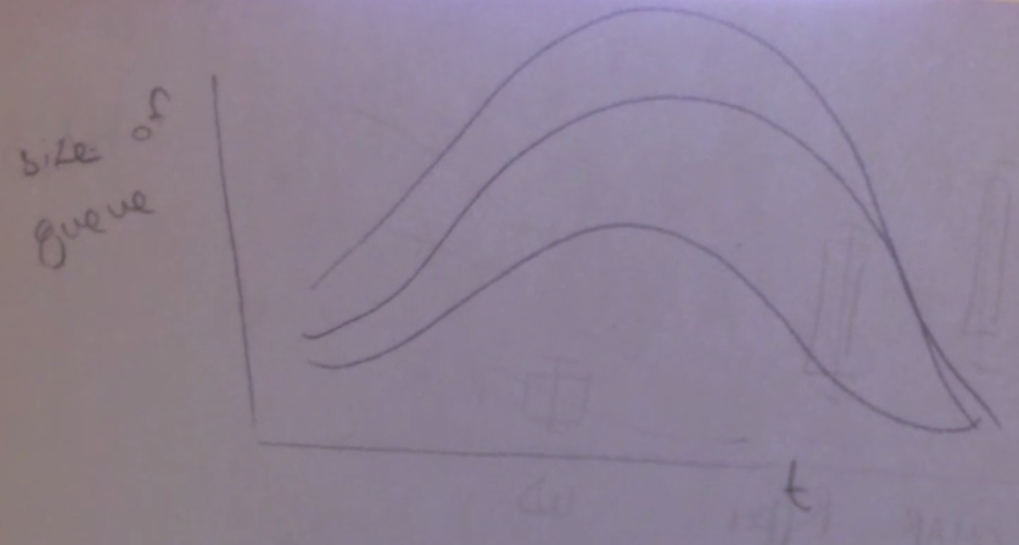
\includegraphics[width=0.65\textwidth]{figs/sketch-queue-size.png}
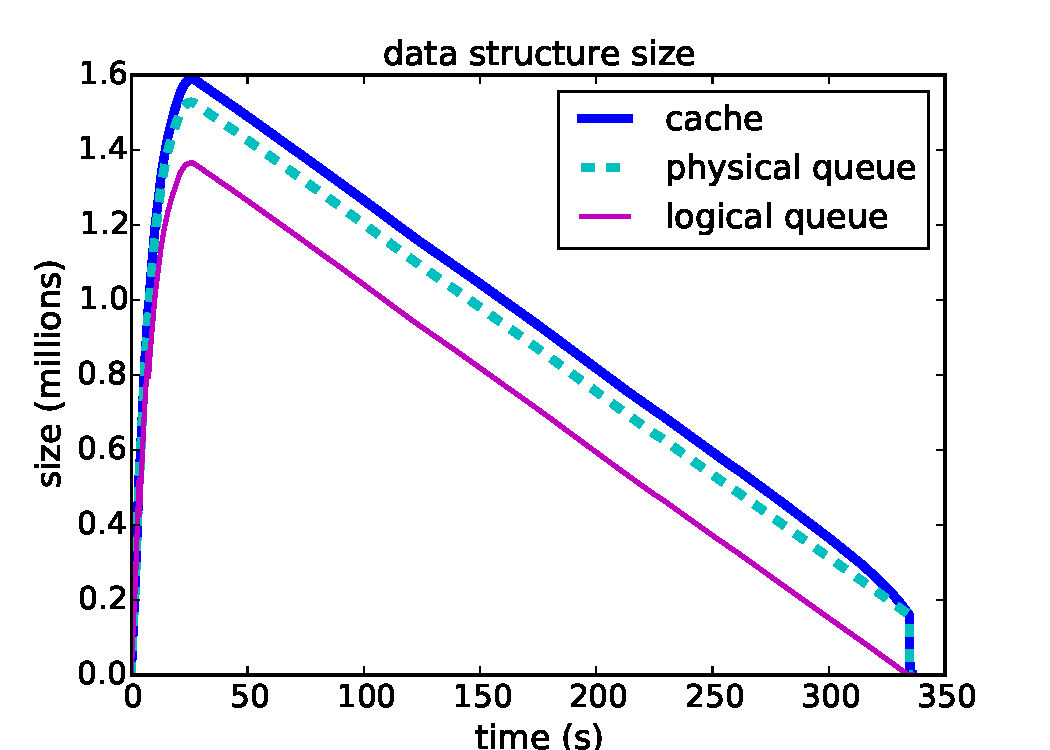
\includegraphics[width=0.8\textwidth]{figs/ela_compas-queue-cache-size-insertions.pdf}
\end{center}
\caption{Cache and queue data structure sizes and insertions.
%
The top plot shows the sizes of the cache and queue data structures,
as a function of wall clock time.
%
The number of nodes in the cache (solid black line) is an
upper bound on the number of elements in the physical queue
(dotted gray line), since the physical queue elements only
correspond to the cache trie data structure's leaf nodes
plus disconnected cache nodes that have been marked for deletion.
%
The queue's physical size is an upper bound on its
logical size (solid blue line), which doesn't include nodes
that have been marked for deletion.
%
The bottom plot shows the cumulative number of cache insertions,
which is equivalent to the cumulative number of queue insertions,
as a function of wall clock time.
}
\label{fig:queue-cache-size-insertions}
\end{figure}
\end{arxiv}

\begin{figure}[t!]
\begin{center}
\begin{arxiv}
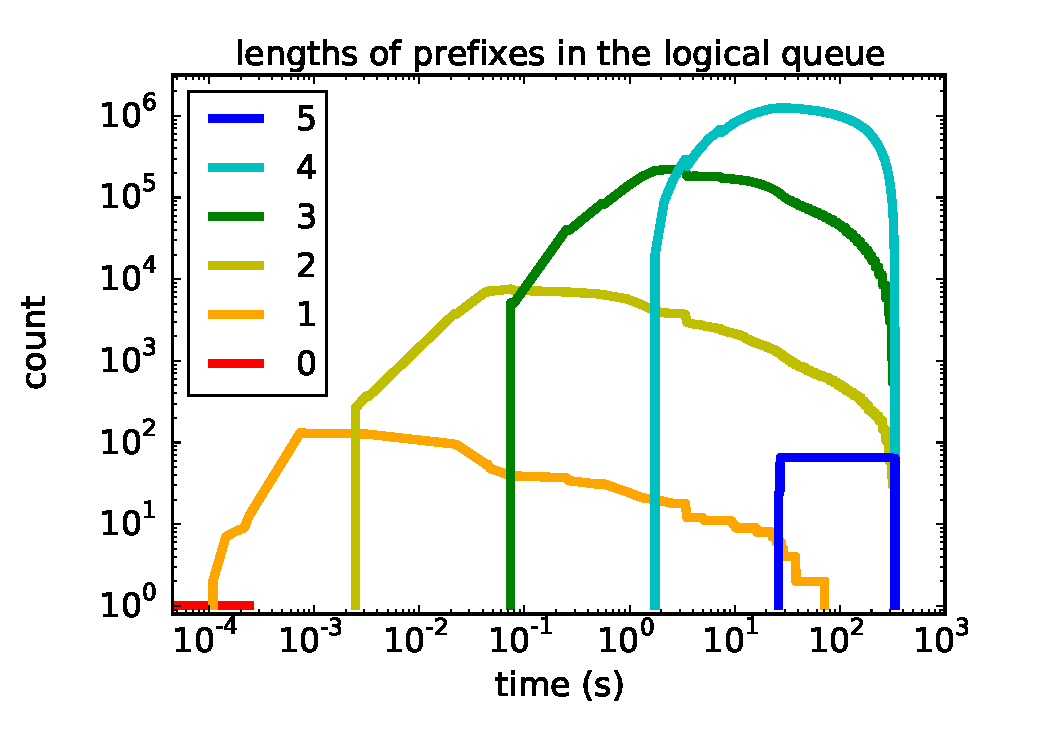
\includegraphics[width=0.8\textwidth]{figs/ela_compas-queue.pdf}
\end{arxiv}
\begin{kdd}
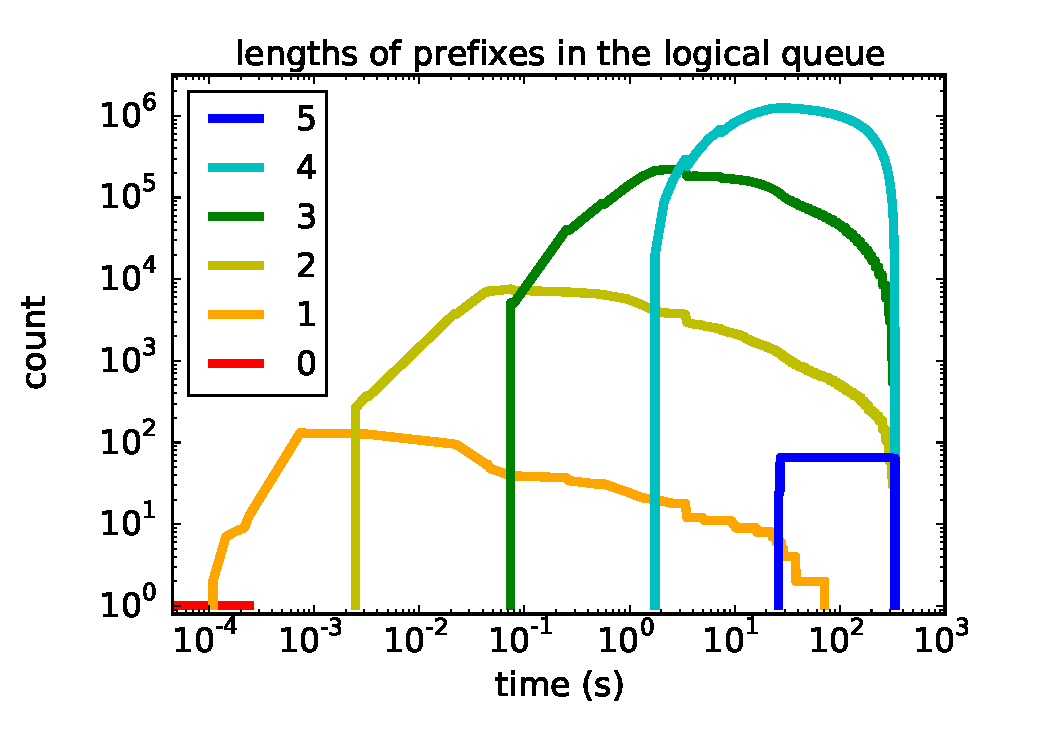
\includegraphics[width=0.5\textwidth]{figs/ela_compas-queue.pdf}
\end{kdd}
\end{center}
\caption{Logical queue composition.
}
\label{fig:queue}
\end{figure}

\begin{figure}[t!]
\begin{center}
%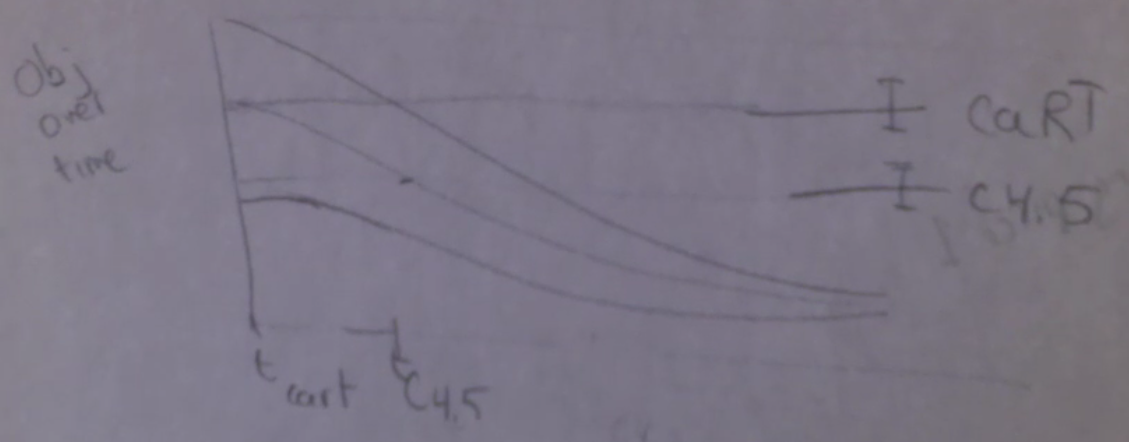
\includegraphics[width=0.65\textwidth]{figs/sketch-objective.png}
\begin{arxiv}
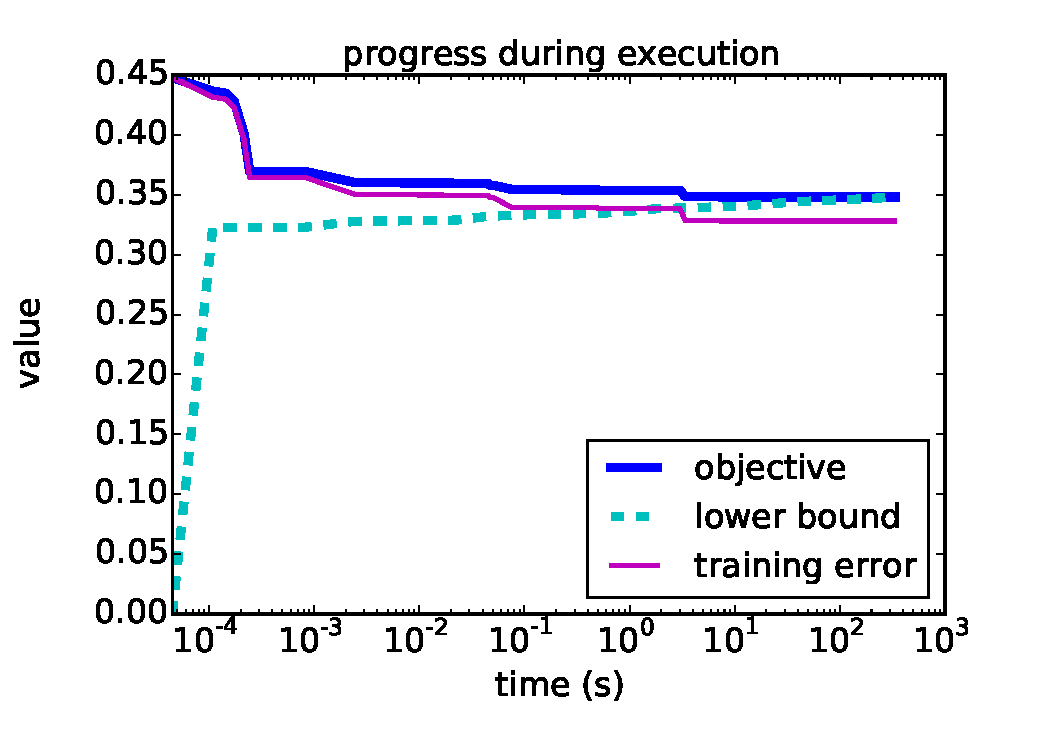
\includegraphics[width=0.8\textwidth]{figs/ela_compas-objective.pdf}
\end{arxiv}
\begin{kdd}
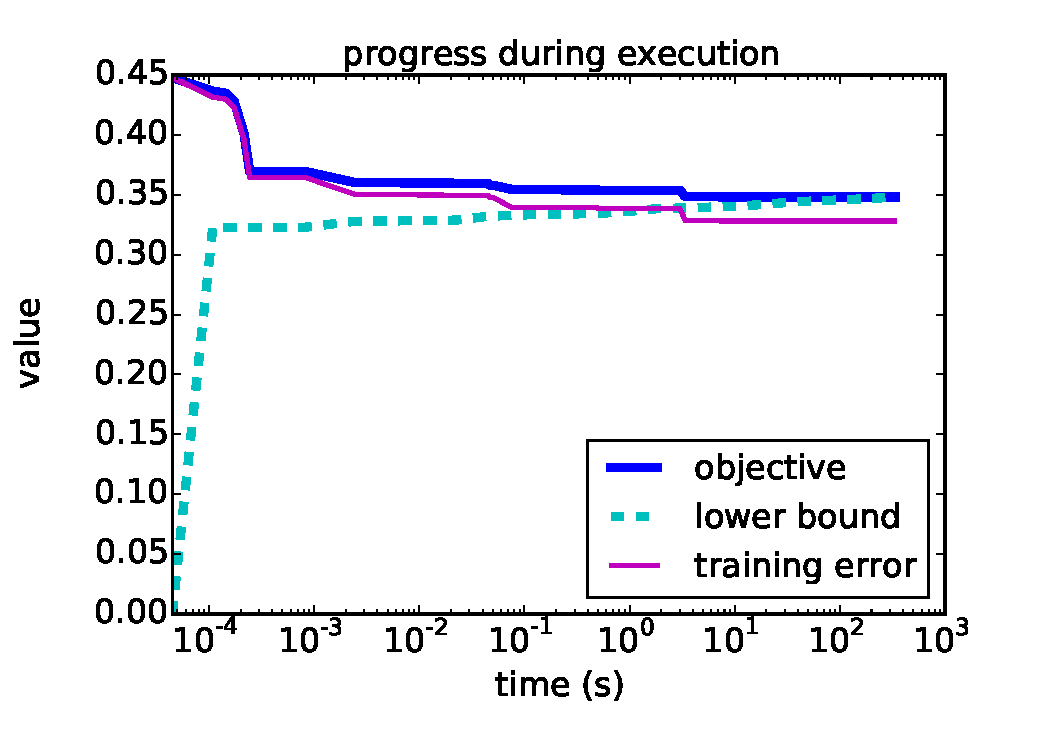
\includegraphics[width=0.5\textwidth]{figs/ela_compas-objective.pdf}
\end{kdd}
\end{center}
\caption{Objective value as a function of wall clock time.
%
The top plot shows the entire execution, and the bottom plot
highlights the optimization phase, from the start of execution
to the time at which the optimal value is achieved.
%
The cyan circle indicates the objective value after a single iteration,
and the magenta square indicates the time at which the optimum
is achieved, as well as its value.
%
Missing: horizontal lines and x-ticks for CART and C4.5.}
\label{fig:objective}
\end{figure}

\begin{figure}[t!]
\begin{center}
%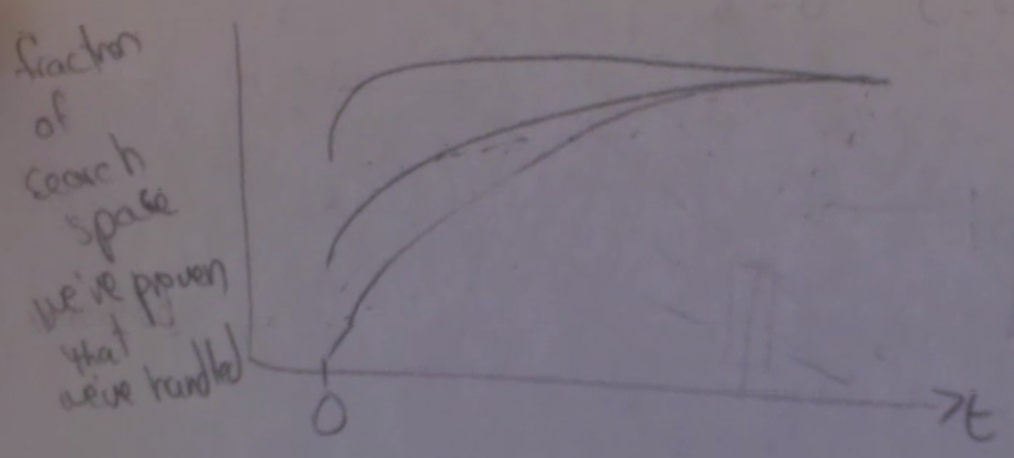
\includegraphics[width=0.65\textwidth]{figs/sketch-search-space.png}
\begin{arxiv}
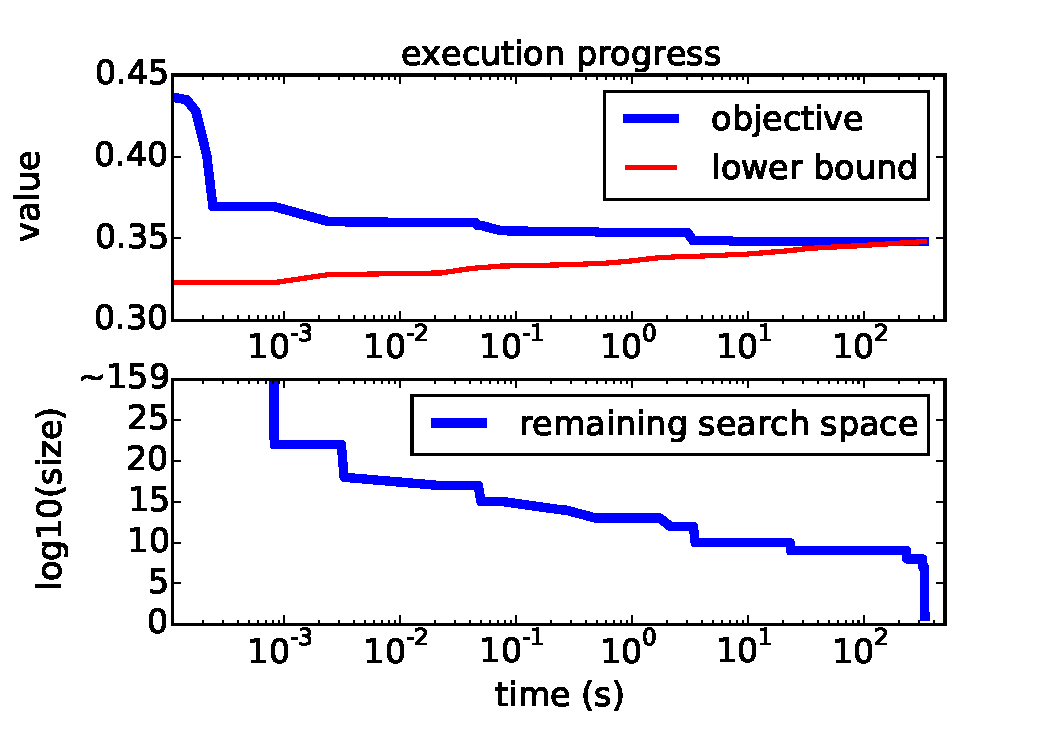
\includegraphics[width=0.8\textwidth]{figs/ela_compas-remaining-space.pdf}
\end{arxiv}
\begin{kdd}
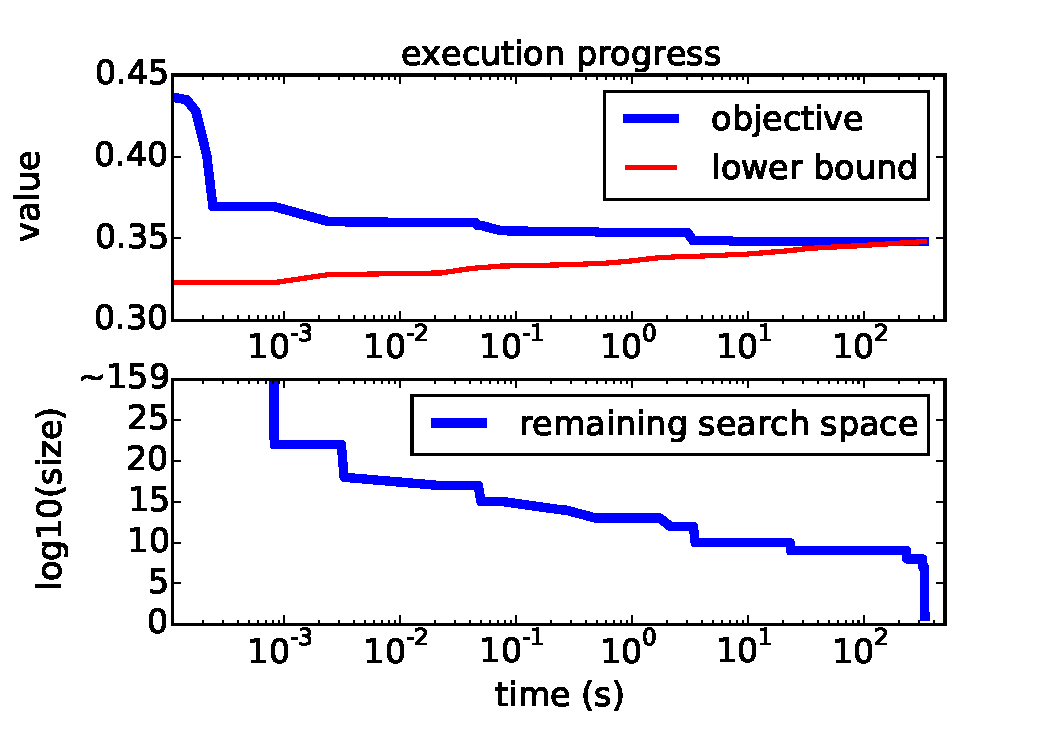
\includegraphics[width=0.5\textwidth]{figs/ela_compas-remaining-space.pdf}
\end{kdd}
\end{center}
\caption{The logarithm (base 10) of the upper bound
from Proposition~\ref{prop:remaining-eval-coarse}
on the size of the remaining search space,
as a function of wall clock time.
%
This bound depends on the total number of available rules,
as well as two dynamic quantities:
the current best objective value,
and the histogram of logical queue elements,
partitioned by prefix length.
}
\label{fig:search-space}
\end{figure}

\begin{arxiv}
\begin{figure}[t!]
\begin{center}
%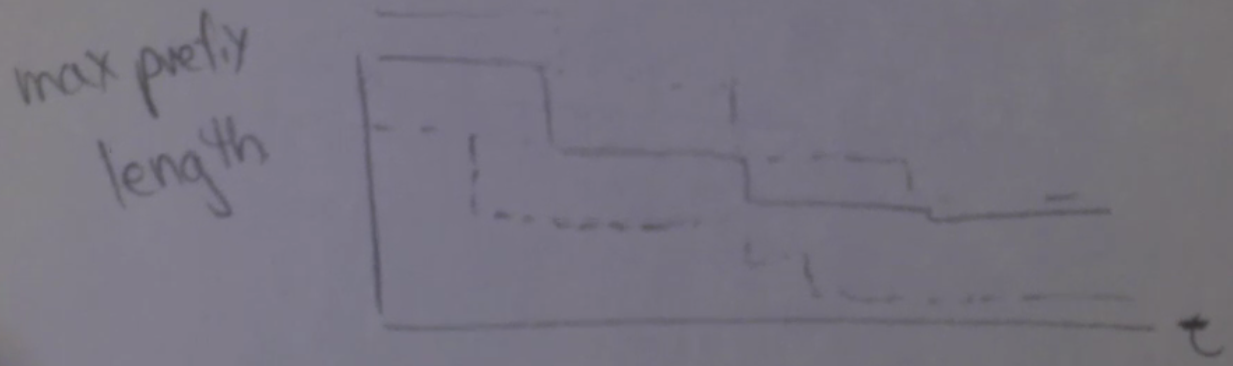
\includegraphics[width=0.65\textwidth]{figs/sketch-max-length.png}
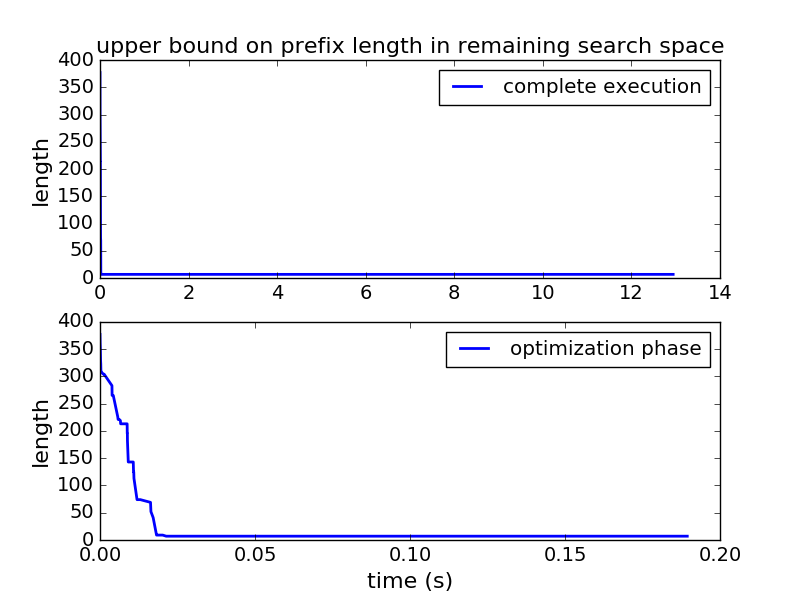
\includegraphics[width=0.8\textwidth]{figs/ela-max-length-check.png}
\end{center}
\caption{Max prefix length over time (computed from objective value)}
\label{fig:max-length}
\end{figure}

\begin{figure}[t!]
\begin{center}
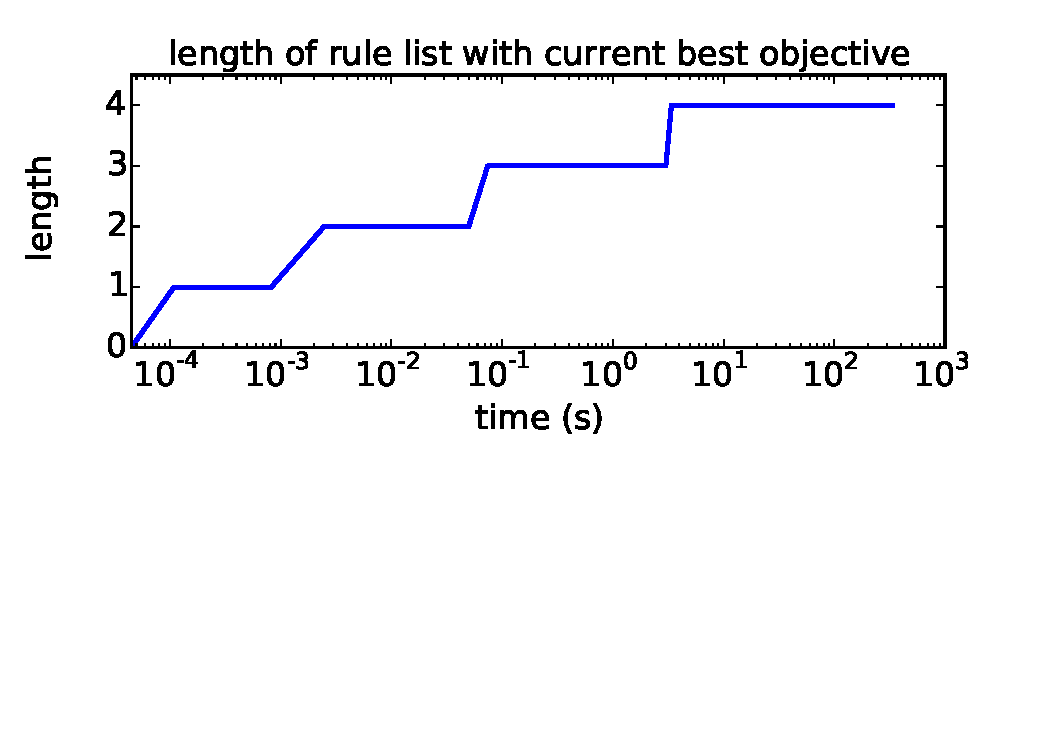
\includegraphics[width=0.8\textwidth]{figs/ela_compas-prefix-length.pdf}
\end{center}
\caption{Best prefix length over time}
\label{fig:prefix-length}
\end{figure}
\end{arxiv}


%\section{Introduction}

The \textit{proceedings} are the records of a conference\footnote{This
  is a footnote}.  ACM seeks
to give these conference by-products a uniform, high-quality
appearance.  To do this, ACM has some rigid requirements for the
format of the proceedings documents: there is a specified format
(balanced double columns), a specified set of fonts (Arial or
Helvetica and Times Roman) in certain specified sizes, a specified
live area, centered on the page, specified size of margins, specified
column width and gutter size.

\section{The Body of The Paper}
Typically, the body of a paper is organized into a hierarchical
structure, with numbered or unnumbered headings for sections,
subsections, sub-subsections, and even smaller sections.  The command
\texttt{{\char'134}section} that precedes this paragraph is part of
such a hierarchy.\footnote{This is a footnote.} \LaTeX\ handles the
numbering and placement of these headings for you, when you use the
appropriate heading commands around the titles of the headings.  If
you want a sub-subsection or smaller part to be unnumbered in your
output, simply append an asterisk to the command name.  Examples of
both numbered and unnumbered headings will appear throughout the
balance of this sample document.

Because the entire article is contained in the \textbf{document}
environment, you can indicate the start of a new paragraph with a
blank line in your input file; that is why this sentence forms a
separate paragraph.

\subsection{Type Changes and {\itshape Special} Characters}

We have already seen several typeface changes in this sample.  You can
indicate italicized words or phrases in your text with the command
\texttt{{\char'134}textit}; emboldening with the command
\texttt{{\char'134}textbf} and typewriter-style (for instance, for
computer code) with \texttt{{\char'134}texttt}.  But remember, you do
not have to indicate typestyle changes when such changes are part of
the \textit{structural} elements of your article; for instance, the
heading of this subsection will be in a sans serif\footnote{Another
  footnote, here.  Let's make this a rather short one to see how it
  looks.} typeface, but that is handled by the document class file.
Take care with the use of\footnote{A third, and last, footnote.}  the
curly braces in typeface changes; they mark the beginning and end of
the text that is to be in the different typeface.

You can use whatever symbols, accented characters, or non-English
characters you need anywhere in your document; you can find a complete
list of what is available in the \textit{\LaTeX\ User's Guide}
\cite{Lamport:LaTeX}.

\subsection{Math Equations}
You may want to display math equations in three distinct styles:
inline, numbered or non-numbered display.  Each of
the three are discussed in the next sections.

\subsubsection{Inline (In-text) Equations}
A formula that appears in the running text is called an
inline or in-text formula.  It is produced by the
\textbf{math} environment, which can be
invoked with the usual \texttt{{\char'134}begin\,\ldots{\char'134}end}
construction or with the short form \texttt{\$\,\ldots\$}. You
can use any of the symbols and structures,
from $\alpha$ to $\omega$, available in
\LaTeX~\cite{Lamport:LaTeX}; this section will simply show a
few examples of in-text equations in context. Notice how
this equation:
\begin{math}
  \lim_{n\rightarrow \infty}x=0
\end{math},
set here in in-line math style, looks slightly different when
set in display style.  (See next section).

\subsubsection{Display Equations}
A numbered display equation---one set off by vertical space from the
text and centered horizontally---is produced by the \textbf{equation}
environment. An unnumbered display equation is produced by the
\textbf{displaymath} environment.

Again, in either environment, you can use any of the symbols
and structures available in \LaTeX\@; this section will just
give a couple of examples of display equations in context.
First, consider the equation, shown as an inline equation above:
\begin{equation}
  \lim_{n\rightarrow \infty}x=0
\end{equation}
Notice how it is formatted somewhat differently in
the \textbf{displaymath}
environment.  Now, we'll enter an unnumbered equation:
\begin{displaymath}
  \sum_{i=0}^{\infty} x + 1
\end{displaymath}
and follow it with another numbered equation:
\begin{equation}
  \sum_{i=0}^{\infty}x_i=\int_{0}^{\pi+2} f
\end{equation}
just to demonstrate \LaTeX's able handling of numbering.

\subsection{Citations}
Citations to articles~\cite{bowman:reasoning,
clark:pct, braams:babel, herlihy:methodology},
conference proceedings~\cite{clark:pct} or maybe
books \cite{Lamport:LaTeX, salas:calculus} listed
in the Bibliography section of your
article will occur throughout the text of your article.
You should use BibTeX to automatically produce this bibliography;
you simply need to insert one of several citation commands with
a key of the item cited in the proper location in
the \texttt{.tex} file~\cite{Lamport:LaTeX}.
The key is a short reference you invent to uniquely
identify each work; in this sample document, the key is
the first author's surname and a
word from the title.  This identifying key is included
with each item in the \texttt{.bib} file for your article.

The details of the construction of the \texttt{.bib} file
are beyond the scope of this sample document, but more
information can be found in the \textit{Author's Guide},
and exhaustive details in the \textit{\LaTeX\ User's
Guide} by Lamport~\shortcite{Lamport:LaTeX}.


This article shows only the plainest form
of the citation command, using \texttt{{\char'134}cite}.

\subsection{Tables}
Because tables cannot be split across pages, the best
placement for them is typically the top of the page
nearest their initial cite.  To
ensure this proper ``floating'' placement of tables, use the
environment \textbf{table} to enclose the table's contents and
the table caption.  The contents of the table itself must go
in the \textbf{tabular} environment, to
be aligned properly in rows and columns, with the desired
horizontal and vertical rules.  Again, detailed instructions
on \textbf{tabular} material
are found in the \textit{\LaTeX\ User's Guide}.

Immediately following this sentence is the point at which
Table~\ref{tab:freq} is included in the input file; compare the
placement of the table here with the table in the printed
output of this document.

\begin{table}
  \caption{Frequency of Special Characters}
  \label{tab:freq}
  \begin{tabular}{ccl}
    \toprule
    Non-English or Math&Frequency&Comments\\
    \midrule
    \O & 1 in 1,000& For Swedish names\\
    $\pi$ & 1 in 5& Common in math\\
    \$ & 4 in 5 & Used in business\\
    $\Psi^2_1$ & 1 in 40,000& Unexplained usage\\
  \bottomrule
\end{tabular}
\end{table}

To set a wider table, which takes up the whole width of the page's
live area, use the environment \textbf{table*} to enclose the table's
contents and the table caption.  As with a single-column table, this
wide table will ``float'' to a location deemed more desirable.
Immediately following this sentence is the point at which
Table~\ref{tab:commands} is included in the input file; again, it is
instructive to compare the placement of the table here with the table
in the printed output of this document.


\begin{table*}
  \caption{Some Typical Commands}
  \label{tab:commands}
  \begin{tabular}{ccl}
    \toprule
    Command &A Number & Comments\\
    \midrule
    \texttt{{\char'134}author} & 100& Author \\
    \texttt{{\char'134}table}& 300 & For tables\\
    \texttt{{\char'134}table*}& 400& For wider tables\\
    \bottomrule
  \end{tabular}
\end{table*}
% end the environment with {table*}, NOTE not {table}!

It is strongly recommended to use the package booktabs~\cite{Fear05}
and follow its main principles of typography with respect to tables:
\begin{enumerate}
\item Never, ever use vertical rules.
\item Never use double rules.
\end{enumerate}
It is also a good idea not to overuse horizontal rules.


\subsection{Figures}

Like tables, figures cannot be split across pages; the best placement
for them is typically the top or the bottom of the page nearest their
initial cite.  To ensure this proper ``floating'' placement of
figures, use the environment \textbf{figure} to enclose the figure and
its caption.

This sample document contains examples of \texttt{.eps} files to be
displayable with \LaTeX.  If you work with pdf\LaTeX, use files in the
\texttt{.pdf} format.  Note that most modern \TeX\ systems will convert
\texttt{.eps} to \texttt{.pdf} for you on the fly.  More details on
each of these are found in the \textit{Author's Guide}.

\begin{figure}
\includegraphics{fly}
\caption{A sample black and white graphic.}
\end{figure}

\begin{figure}
\includegraphics[height=1in, width=1in]{fly}
\caption{A sample black and white graphic
that has been resized with the \texttt{includegraphics} command.}
\end{figure}


As was the case with tables, you may want a figure that spans two
columns.  To do this, and still to ensure proper ``floating''
placement of tables, use the environment \textbf{figure*} to enclose
the figure and its caption.  And don't forget to end the environment
with \textbf{figure*}, not \textbf{figure}!

\begin{figure*}
\includegraphics{flies}
\caption{A sample black and white graphic
that needs to span two columns of text.}
\end{figure*}


\begin{figure}
\includegraphics[height=1in, width=1in]{rosette}
\caption{A sample black and white graphic that has
been resized with the \texttt{includegraphics} command.}
\end{figure}

\subsection{Theorem-like Constructs}

Other common constructs that may occur in your article are the forms
for logical constructs like theorems, axioms, corollaries and proofs.
ACM uses two types of these constructs:  theorem-like and
definition-like.

Here is a theorem:
\begin{theorem}
  Let $f$ be continuous on $[a,b]$.  If $G$ is
  an antiderivative for $f$ on $[a,b]$, then
  \begin{displaymath}
    \int^b_af(t)\,dt = G(b) - G(a).
  \end{displaymath}
\end{theorem}

Here is a definition:
\begin{definition}
  If $z$ is irrational, then by $e^z$ we mean the
  unique number that has
  logarithm $z$:
  \begin{displaymath}
    \log e^z = z.
  \end{displaymath}
\end{definition}

The pre-defined theorem-like constructs are \textbf{theorem},
\textbf{conjecture}, \textbf{proposition}, \textbf{lemma} and
\textbf{corollary}.  The pre-defined de\-fi\-ni\-ti\-on-like constructs are
\textbf{example} and \textbf{definition}.  You can add your own
constructs using the \textsl{amsthm} interface~\cite{Amsthm15}.  The
styles used in the \verb|\theoremstyle| command are \textbf{acmplain}
and \textbf{acmdefinition}.

Another construct is \textbf{proof}, for example,

\begin{proof}
  Suppose on the contrary there exists a real number $L$ such that
  \begin{displaymath}
    \lim_{x\rightarrow\infty} \frac{f(x)}{g(x)} = L.
  \end{displaymath}
  Then
  \begin{displaymath}
    l=\lim_{x\rightarrow c} f(x)
    = \lim_{x\rightarrow c}
    \left[ g{x} \cdot \frac{f(x)}{g(x)} \right ]
    = \lim_{x\rightarrow c} g(x) \cdot \lim_{x\rightarrow c}
    \frac{f(x)}{g(x)} = 0\cdot L = 0,
  \end{displaymath}
  which contradicts our assumption that $l\neq 0$.
\end{proof}

\section{Conclusions}
This paragraph will end the body of this sample document.
Remember that you might still have Acknowledgments or
Appendices; brief samples of these
follow.  There is still the Bibliography to deal with; and
we will make a disclaimer about that here: with the exception
of the reference to the \LaTeX\ book, the citations in
this paper are to articles which have nothing to
do with the present subject and are used as
examples only.
%\end{document}  % This is where a 'short' article might terminate



\appendix
%Appendix A
\section{Headings in Appendices}
The rules about hierarchical headings discussed above for
the body of the article are different in the appendices.
In the \textbf{appendix} environment, the command
\textbf{section} is used to
indicate the start of each Appendix, with alphabetic order
designation (i.e., the first is A, the second B, etc.) and
a title (if you include one).  So, if you need
hierarchical structure
\textit{within} an Appendix, start with \textbf{subsection} as the
highest level. Here is an outline of the body of this
document in Appendix-appropriate form:
\subsection{Introduction}
\subsection{The Body of the Paper}
\subsubsection{Type Changes and  Special Characters}
\subsubsection{Math Equations}
\paragraph{Inline (In-text) Equations}
\paragraph{Display Equations}
\subsubsection{Citations}
\subsubsection{Tables}
\subsubsection{Figures}
\subsubsection{Theorem-like Constructs}
\subsubsection*{A Caveat for the \TeX\ Expert}
\subsection{Conclusions}
\subsection{References}
Generated by bibtex from your \texttt{.bib} file.  Run latex,
then bibtex, then latex twice (to resolve references)
to create the \texttt{.bbl} file.  Insert that \texttt{.bbl}
file into the \texttt{.tex} source file and comment out
the command \texttt{{\char'134}thebibliography}.
% This next section command marks the start of
% Appendix B, and does not continue the present hierarchy
\section{More Help for the Hardy}

Of course, reading the source code is always useful.  The file
\path{acmart.pdf} contains both the user guide and the commented
code.

\begin{acks}
  The authors would like to thank Dr. Yuhua Li for providing the
  matlab code of  the \textit{BEPS} method. 

  The authors would also like to thank the anonymous referees for
  their valuable comments and helpful suggestions. The work is
  supported by the \grantsponsor{GS501100001809}{National Natural
    Science Foundation of
    China}{http://dx.doi.org/10.13039/501100001809} under Grant
  No.:~\grantnum{GS501100001809}{61273304}
  and~\grantnum[http://www.nnsf.cn/youngscientsts]{GS501100001809}{Young
    Scientsts' Support Program}.

\end{acks}


\bibliographystyle{ACM-Reference-Format}
\bibliography{../paper/refs} 

\end{document}
